\documentclass[11pt]{beamer}
\usepackage[utf8]{inputenc}
\usepackage[T1]{fontenc}
\usepackage{lmodern}
\usepackage[english]{babel}
\usepackage{amsmath}
\usepackage{amsfonts}
\usepackage{amssymb}
\usepackage{graphicx}
\usepackage{hyperref}
\usepackage{color}

\usecolortheme{solarized}
%\usecolortheme[dark]{solarized}

\graphicspath{{img/}}

\begin{document}
	\setbeamertemplate{caption}{\raggedright\insertcaption\par}	% Get rid of "Figure:" label in figures
	\author{ASULUG}
	\title{What is Linux and How Do I Get It Onto My Computer?}
	\subtitle{How to Choose a Distribution}
	\logo{
\includegraphics[width=.2\textwidth]{asulug-logo.png}}
	\institute{Arizona State University}
	%\date{}
	%\subject{}
	%\setbeamercovered{transparent}
	%\setbeamertemplate{navigation symbols}{}
	\begin{frame}[plain]
	\maketitle
	\begin{figure}
		
\includegraphics[scale=2]{asulug-logo.png}
	\end{figure}
	Made with \LaTeX
\end{frame}

\begin{frame}{History}
	\begin{columns}
		\begin{column}{0.5\textwidth}
			\begin{itemize}
				\item \textbf{1969:} Ken Thompson and Dennis Ritchie created Unix Bell Labs, written in PDP-7 assembly language.
				\item \textbf{1972:} The C language was developed by Ritchie and colleague Brian Kernighan using Unix.
				\item \textbf{1973:} Most of Unix was rewritten in C for portability.
				\item \textbf{Late 70s:} Unix licensed to UC Berkeley (BSD), Microsoft (Xenix), IBM (AIX), HP (HPUX), Sun Microsystems (now Oracle) (Solaris)
			\end{itemize}
		\end{column}
		\begin{column}{0.5\textwidth}
			\begin{figure}
				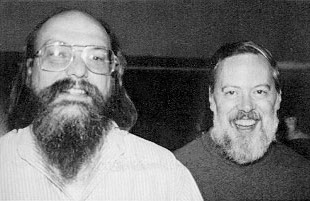
\includegraphics[scale=0.5]{thompson-and-ritchie.png}
				\caption{Thompson (left) and Ritchie (right)}
			\end{figure}
		\end{column}
	\end{columns}
\end{frame}

\begin{frame}{History (\textit{continued})}
	\textbf{\LARGE Influence of Unix:}
	\begin{itemize}
		\item Modular by design
		\item \textbf{Unix Philosophy}: "emphasizes building simple, short, clear, modular, and extensible code that can be easily maintained and repurposed by developers other than its creators."
		\begin{itemize}
			\item Write programs that do one thing and do it well.
			\item Write programs to work together.
			\item Write programs to handle text streams, because that is a universal interface.
		\end{itemize}
		\item Filesystem as main means of communication
		\item Featured a shell scripting and command language (the Unix shell)
	\end{itemize}
\end{frame}

\begin{frame}{History (\textit{continued})}
	\begin{columns}
		\begin{column}{0.5\textwidth}
			\begin{itemize}
				\item \textbf{1983:} \textit{Richard Stallman} started \textit{the GNU project}, aiming to create a free Unix-like operating system.
				\item Stallman created enough software for a fully-functional OS...
				\item ...except the kernel, which he called \textit{Hurd}.
			\end{itemize}
		\end{column}
		\begin{column}{0.5\textwidth}
			\vspace{-10mm}
			\begin{figure}
				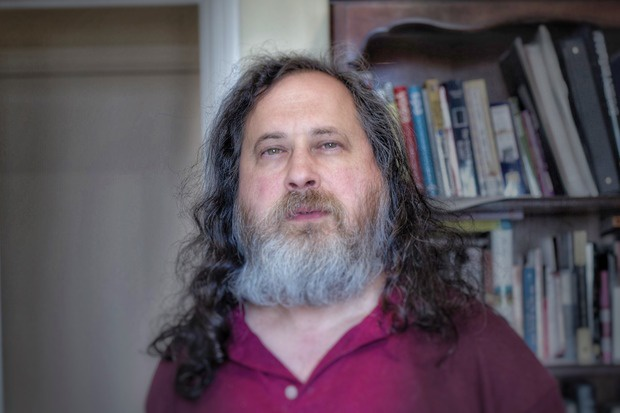
\includegraphics[scale=0.25]{stallman.jpg}
				\caption{Richard Stallman}
			\end{figure}
			\vspace{-6mm}
			\begin{figure}
				
\includegraphics[scale=0.5]{gnu-logo.png}
				\caption{The GNU (GNU's Not Unix) logo}
			\end{figure}
		\end{column}
	\end{columns}
\end{frame}

\begin{frame}{History (\textit{continued})}
	\centering\textbf{\LARGE What is a kernel?}
	\begin{figure}
		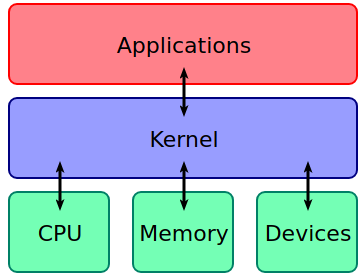
\includegraphics[scale=0.40]{os-diagram.png}
		\caption{\textbf{Kernel:} The main piece and lowest level of an operating system which connects the software applications to the hardware of the computer.}
	\end{figure}
\end{frame}

\begin{frame}{History (\textit{continued})}
	\begin{columns}
		\begin{column}{0.5\textwidth}
			\begin{itemize}
				\item \textbf{1991:} 21-year-old \textit{Linus Torvalds}, a computer science student at the University of Helsinki, Finland, created \textit{Linux}: a free, open source, Unix-like kernel.
				\begin{enumerate}
					\item \textbf{Free:} Free as in \textit{freedom}, not \textit{beer}. One can freely modify the software.
					\item \textbf{Open Source:} The source code of the software is openly available.
				\end{enumerate}
				\item To test his kernel, Torvalds needed application software, so he used that of the GNU project.
			\end{itemize}
		\end{column}
		\begin{column}{0.5\textwidth}
			\vspace{-10mm}
			\begin{figure}
				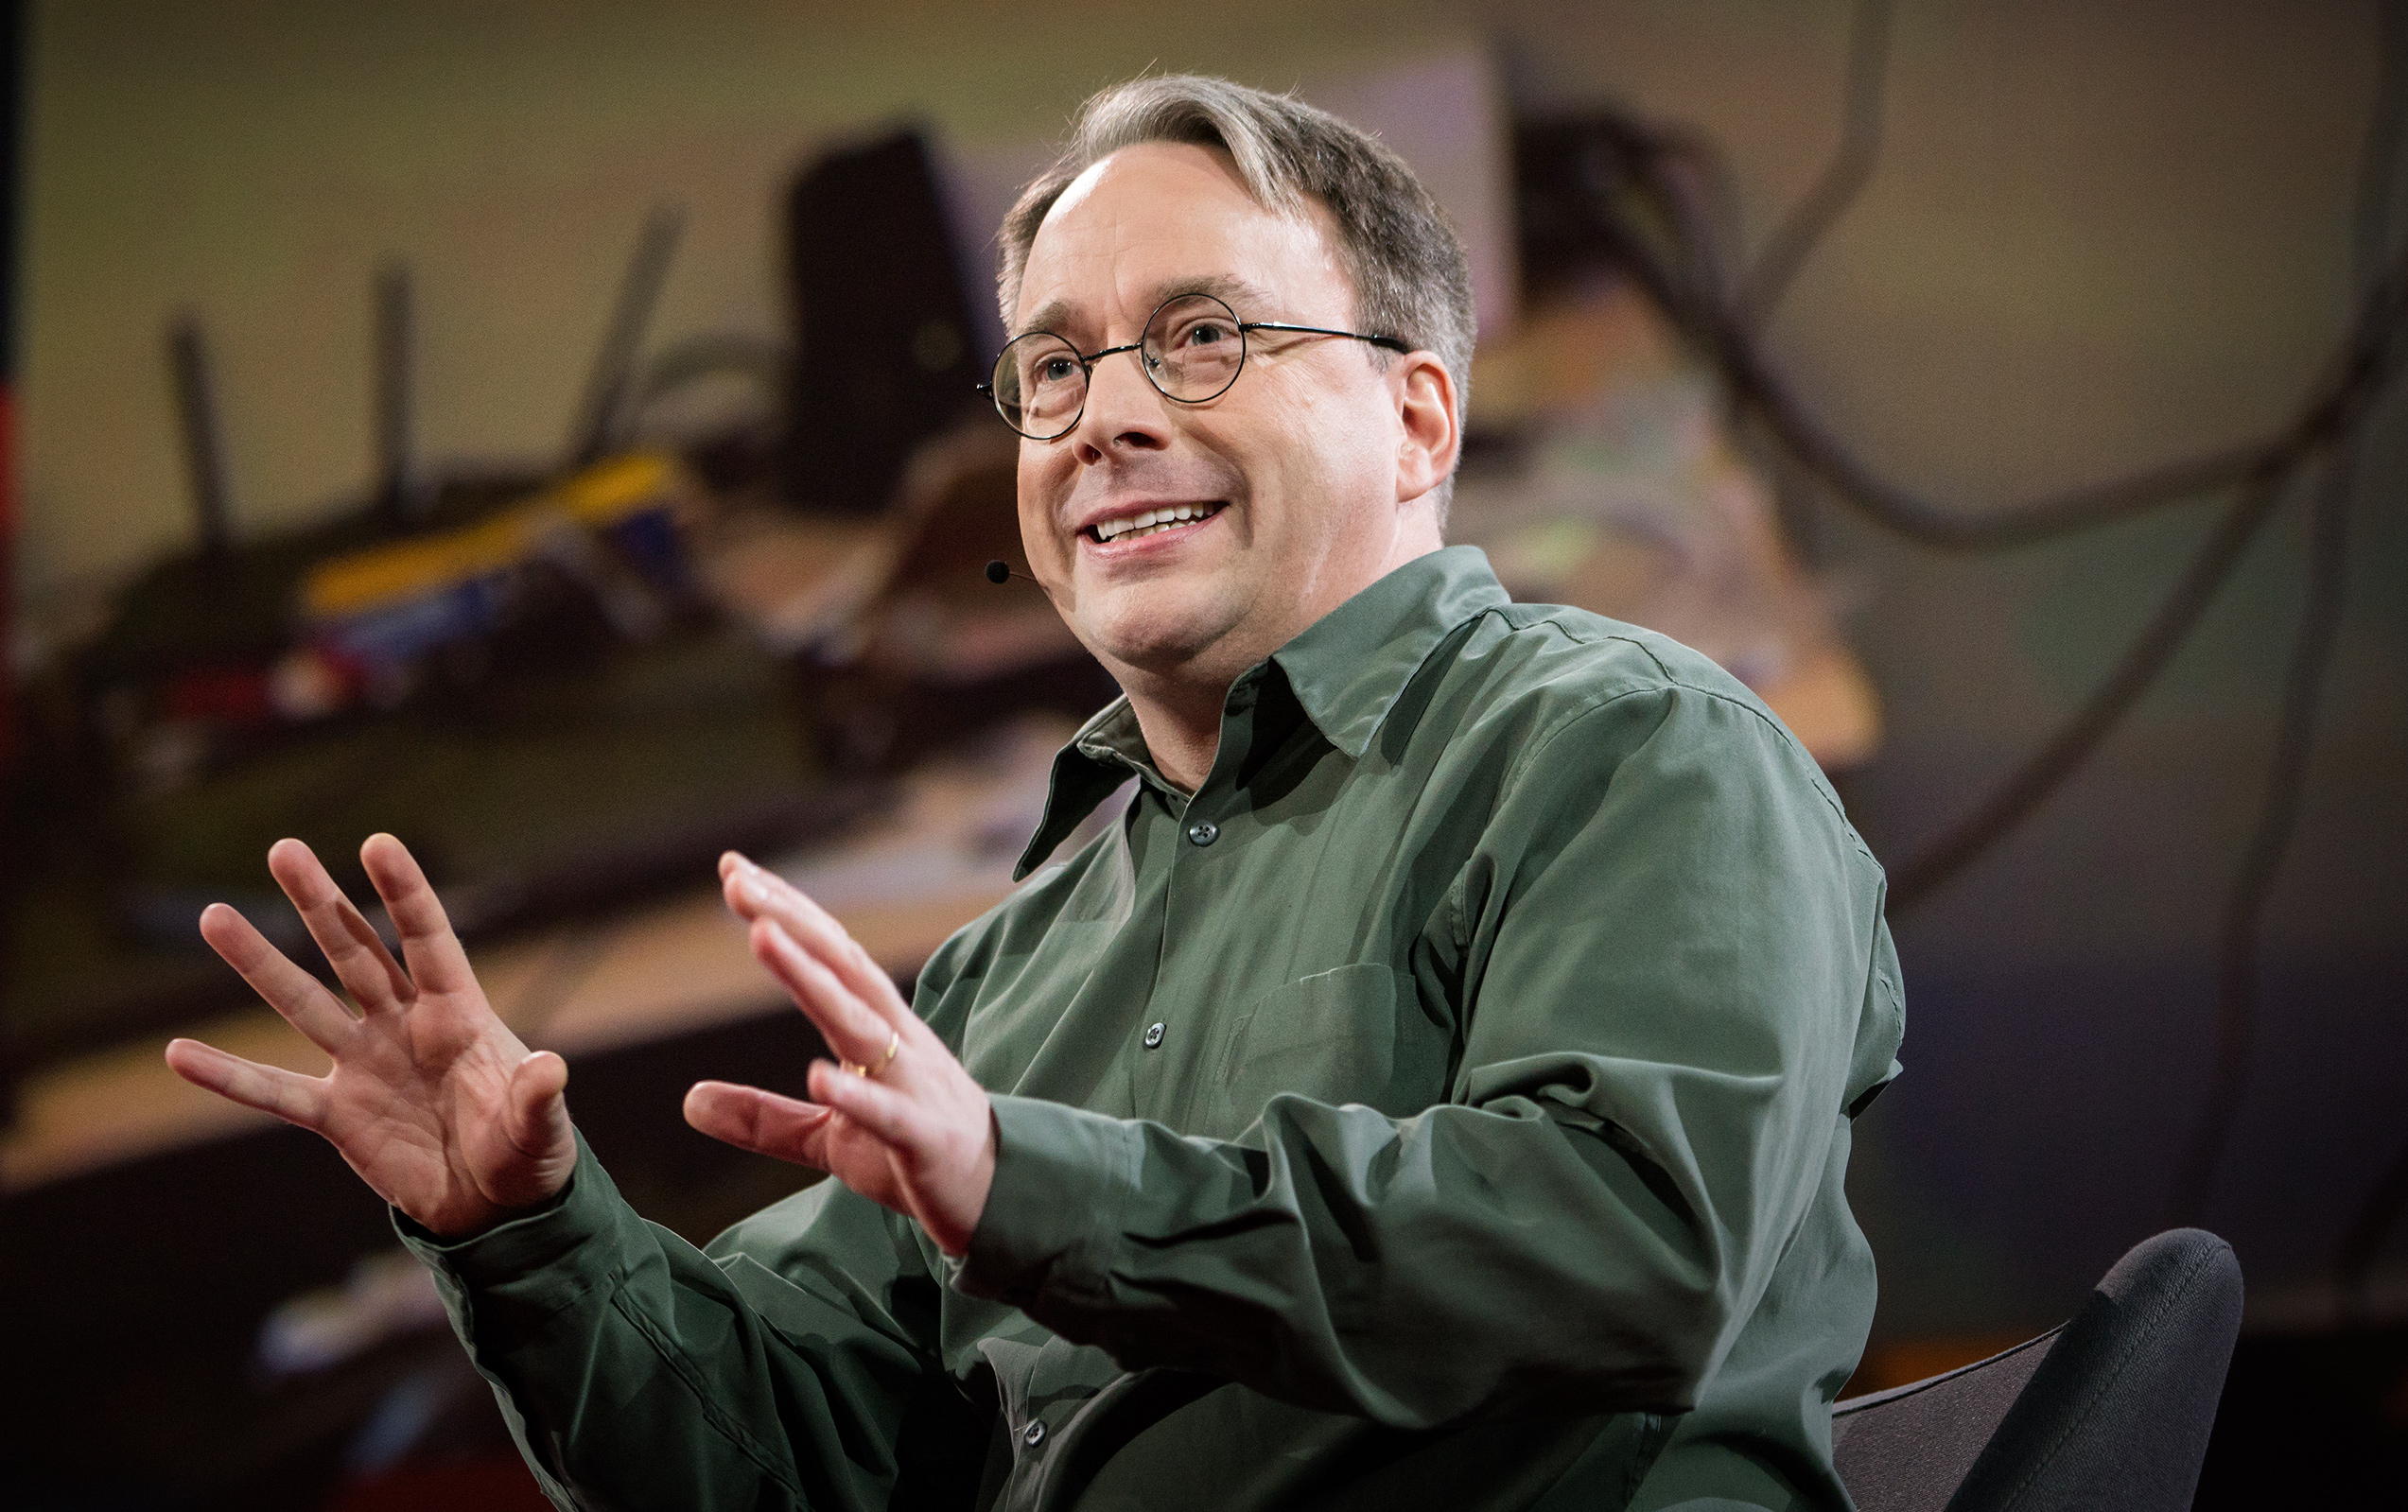
\includegraphics[scale=0.05]{torvalds.jpg}
				\caption{Linus Torvalds}
			\end{figure}
			\vspace{-7mm}
			\begin{figure}
				
\includegraphics[scale=0.25]{tux.png}
				\caption{Tux, the logo and mascot of Linux}
			\end{figure}
		\end{column}
	\end{columns}
\end{frame}

\begin{frame}{So... What Is Linux?}
	\begin{itemize}
		\item \textbf{Linux} itself is a \textit{kernel}.
		\item What people refer to as "Linux operating systems" are actually \textbf{GNU/Linux} bundles, called \textbf{Linux distributions} (\textit{distros} for short).
		\item There are \textit{many} different Linux distributions to choose from!
	\end{itemize}
\end{frame}

\begin{frame}{Why GNU/Linux?}
	\begin{itemize}
		\item<1-> Unlike Windows or MacOS, GNU/Linux is completely free to use.
		\begin{itemize}
			\item<1-> Almost all software for Linux, like Linux itself, is also free and open source.
		\end{itemize}
		\item<2-> Linux's repository and package manager system allows easy installation and upgrading of software applications.
		\begin{itemize}
			\item<2-> Most package managers also cryptographically verify your software for you.
		\end{itemize}
		\item<3-> GNU/Linux offers full customization of the operating to tailor it to the needs of your workflow, etc.
		\begin{itemize}
			\item<3-> Choose a distro for your specific needs
			\item<3-> Choose the software you want to use for certain purposes (e.g. word processor, icon theme, desktop environment)
		\end{itemize}
		\item<4-> A more friendly development environment through its compilers and command-line interface (CLI).
		\item<5-> A plethora of community support.
	\end{itemize}
\end{frame}

\begin{frame}{Which Linux Distribution Should I Choose?}
	\textbf{Check out:} {\color{blue}\url{https://distrowatch.com}} --- a major source for documenting open source operating systems, focusing on Linux and BSD
	\begin{itemize}
		\item \textbf{Current Top 10 Distributions:} \\\hspace{-5mm} \url{https://distrowatch.com/dwres.php?resource=major}
		\item \textbf{All Distributions:} \\\hspace{-5mm} \url{https://distrowatch.com/wiki/index.php/All_Distros}
		\item \textbf{Distribution Popularity (by Page Hit Ranking):} \\\hspace{-5mm} \url{https://distrowatch.com/dwres.php?resource=popularity}
		\item \textbf{DistroWatch Wiki:} \\\hspace{-5mm} \url{https://distrowatch.com/wiki}
	\end{itemize}
	Check each distribution's website!
\end{frame}

\begin{frame}[t]{Factors to Consider}
	\textbf{\LARGE 1. Ease of Use}
	\begin{columns}
		\begin{column}{0.5\textwidth}
			\begin{itemize}
				\item An important factor, especially for beginners.
				\item Your usage: Daily driver? Experimental setup?
				\item Check the distro's website and reviews of the distro.
				\item A relative, quick ranking of distros, easy-to-hard:
				\begin{enumerate}
					\item Linux Mint, Ubuntu, Fedora
					\item Debian, CentOS
					\item Arch Linux
					\item Gentoo Linux
					\item Linux From Scratch
				\end{enumerate}
			\end{itemize}
		\end{column}
		\begin{column}{0.5\textwidth}
			\begin{figure}
				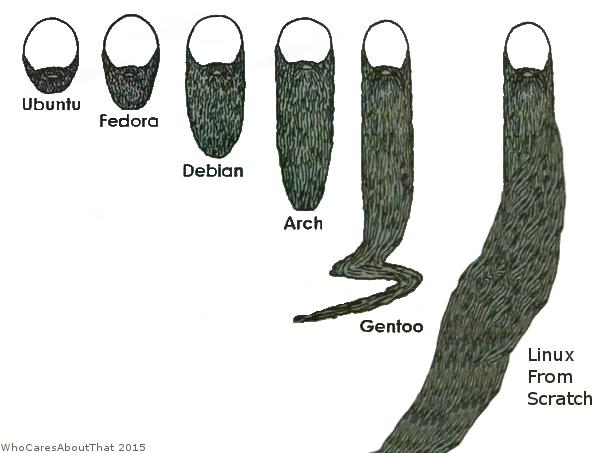
\includegraphics[scale=0.25]{neckbeard-chart.png}
			\end{figure}
		\end{column}
	\end{columns}
\end{frame}

\begin{frame}[t]{Factors to Consider}
	\textbf{\LARGE 2. Stability/Availability}
	\begin{itemize}
		\item Latest software vs. more stable/tested
		\item Rolling-Release vs. Long-Term Support (LTS)
		\item \textbf{Example:} Arch and Gentoo are rolling-release
		\begin{itemize}
			\item More frequent, trickling updates, can be multiple a day if bleeding-edge (Arch)
		\end{itemize}
		\item \textbf{Example:} Ubuntu, Debian, and Red Hat flavors are more on the LTS side of the spectrum
		\begin{itemize}
			\item Less frequent updates, full-system upgrades every certain period of time
		\end{itemize}
		\item \textit{Package Availability}: the more stable distros often come at the cost of lack of package availability for newer packages
	\end{itemize}
\end{frame}

\begin{frame}[t]{Factors to Consider}
	\textbf{\LARGE 3. Support}
	\begin{itemize}
		\item Important for troubleshooting.
		\item Community support vs. company support
		\begin{itemize}
			\item Arch/Ubuntu vs. Red Hat Enterprise Linux (RHEL)
		\end{itemize}
		\item \textbf{Documentation is important!} Some distributions have more support and/or better documentation than others.
		\begin{itemize}
			\item Arch Linux is an extremely well-documented and well-supported distribution with an extensive Wiki.
			\item Content on its Wiki can often be used to solve problems on other distributions.
		\end{itemize}
		\item Popular distributions like Ubuntu and CentOS also have active forums where users can get support from developers and the community of other users.
	\end{itemize}
\end{frame}

\begin{frame}[t]{Factors to Consider}
	\textbf{\LARGE 4. Popularity}
	\begin{itemize}
		\item More popular = more a wider community of users, therefore more community support
		\item Popular distributionss have often been tested on a variety of different hardware
		\begin{itemize}
			\item Ubuntu has distributions for desktop, server, and IoT applications
		\end{itemize}
	\end{itemize}
\end{frame}

\begin{frame}[t]{Factors to Consider}
	\textbf{\LARGE 5. Customizability}
	\begin{itemize}
		\item All Linux distros (that I know of) are customizable.
		\item Ease of customization depends on the distribution.
		\item Distributions that come with a graphical interface like Ubuntu, Debian, OpenSUSE, and CentOS are preconfigured but can be changed.
		\item Some distributions like Arch and Gentoo \textit{do not} come with a graphical interface, leaving the user the choice of which software to install and configure themselves.
		\begin{itemize}
			\item Aimed at experienced users wanting to greatly customize and make efficient their system.
			\item Great for learning and understanding how Linux operating systems work under the hood.
		\end{itemize}
	\end{itemize}
\end{frame}

\begin{frame}[t]{Factors to Consider}
	\textbf{\LARGE 6. Defaults}
	\begin{itemize}
		\item Similar to customizability.
		\item There are several flavors of certain software, like different flavors of ice cream.
		\item For example, KDE, GNOME, and XFCE are three of many Desktop Environments (DEs) with different features.
		\begin{itemize}
			\item Ubuntu comes with GNOME, but you are able to change it for, e.g. KDE. Not so with Windows/Mac!
			\begin{itemize}
				\item If you don't like vanilla ice cream, you could switch to chocolate!
				\item A flavor of Ubuntu exists with KDE already: Kubuntu
			\end{itemize}
			\item If DEs are too much for you, replace it with something more minimal like a Window Manager (WM) such as i3, OpenBox, or Awesome.
			\begin{itemize}
				\item If ice cream is too much for you, you could switch to frozen yogurt!
			\end{itemize}
		\end{itemize}
		\item Linux works this way with all of its applications, even the shell program you use when you interact with the terminal!
	\end{itemize}
\end{frame}

\begin{frame}
	\centering\textbf{\Huge Distributions}
\end{frame}

\begin{frame}{
\includegraphics[scale=0.3]{ubuntu-logo.png} Ubuntu}
	\begin{figure}
		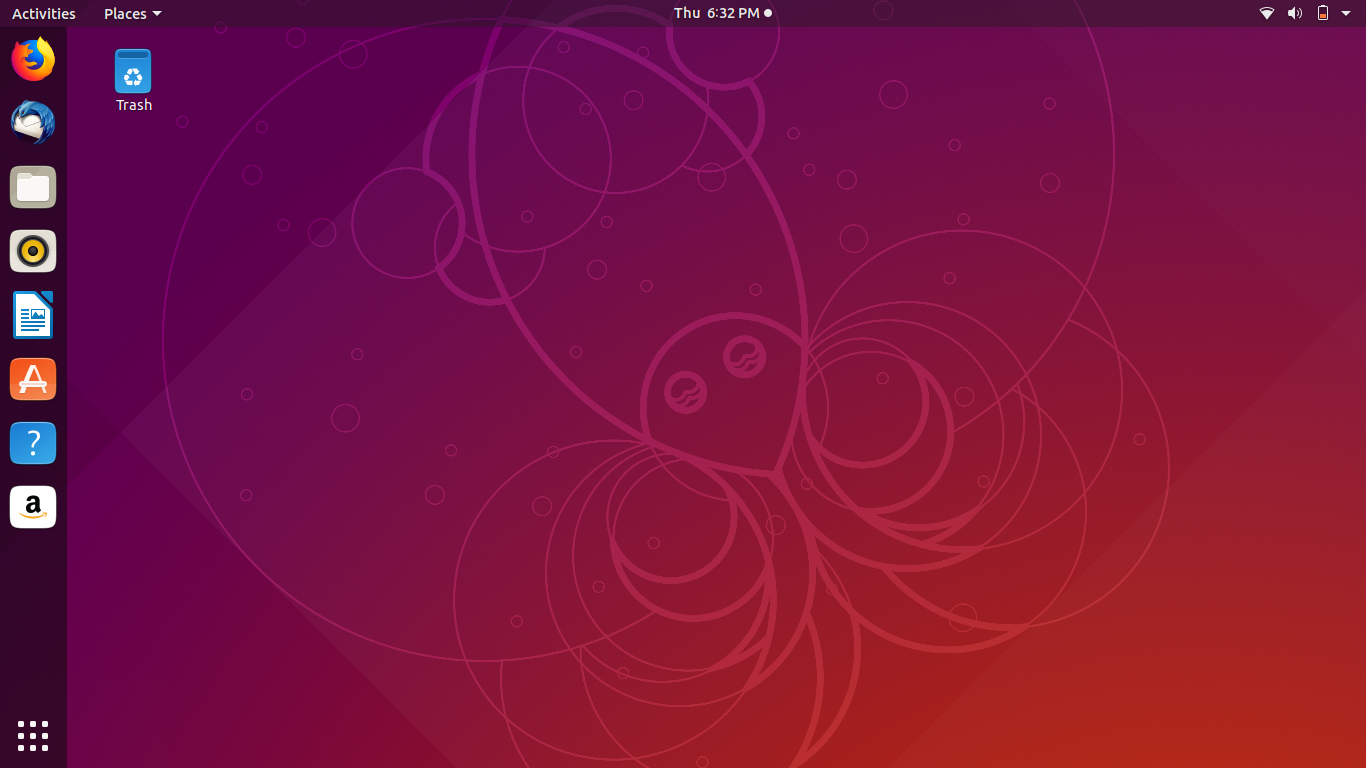
\includegraphics[scale=0.15]{ubuntu-screenshot.png}
	\end{figure}
	\begin{columns}
		\small
		\begin{column}{0.35\textwidth}
			\begin{itemize}
				\item \textbf{Ease of Use:} Easy
				\item \textbf{Stability:} Somewhat Stable
				\item \textbf{Default DE:} GNOME
			\end{itemize}
		\end{column}
		\begin{column}{0.65\textwidth}
			\small
			\textbf{Description:} Owned by Canonical LTD and is based off of Debian, offering three platforms: Desktop, Server, and Core (for IoT).
			\begin{itemize}
				\item Aimed at beginners. Acts similarly to Windows/Mac, making it easier for those transitioning from those platforms.
				\item Package manager is \textit{apt} (Advanced Packaging Tool).
			\end{itemize}
		\end{column}
	\end{columns}
\end{frame}

\begin{frame}{
\includegraphics[scale=0.03]{fedora-logo.png} Fedora}
	\begin{figure}
		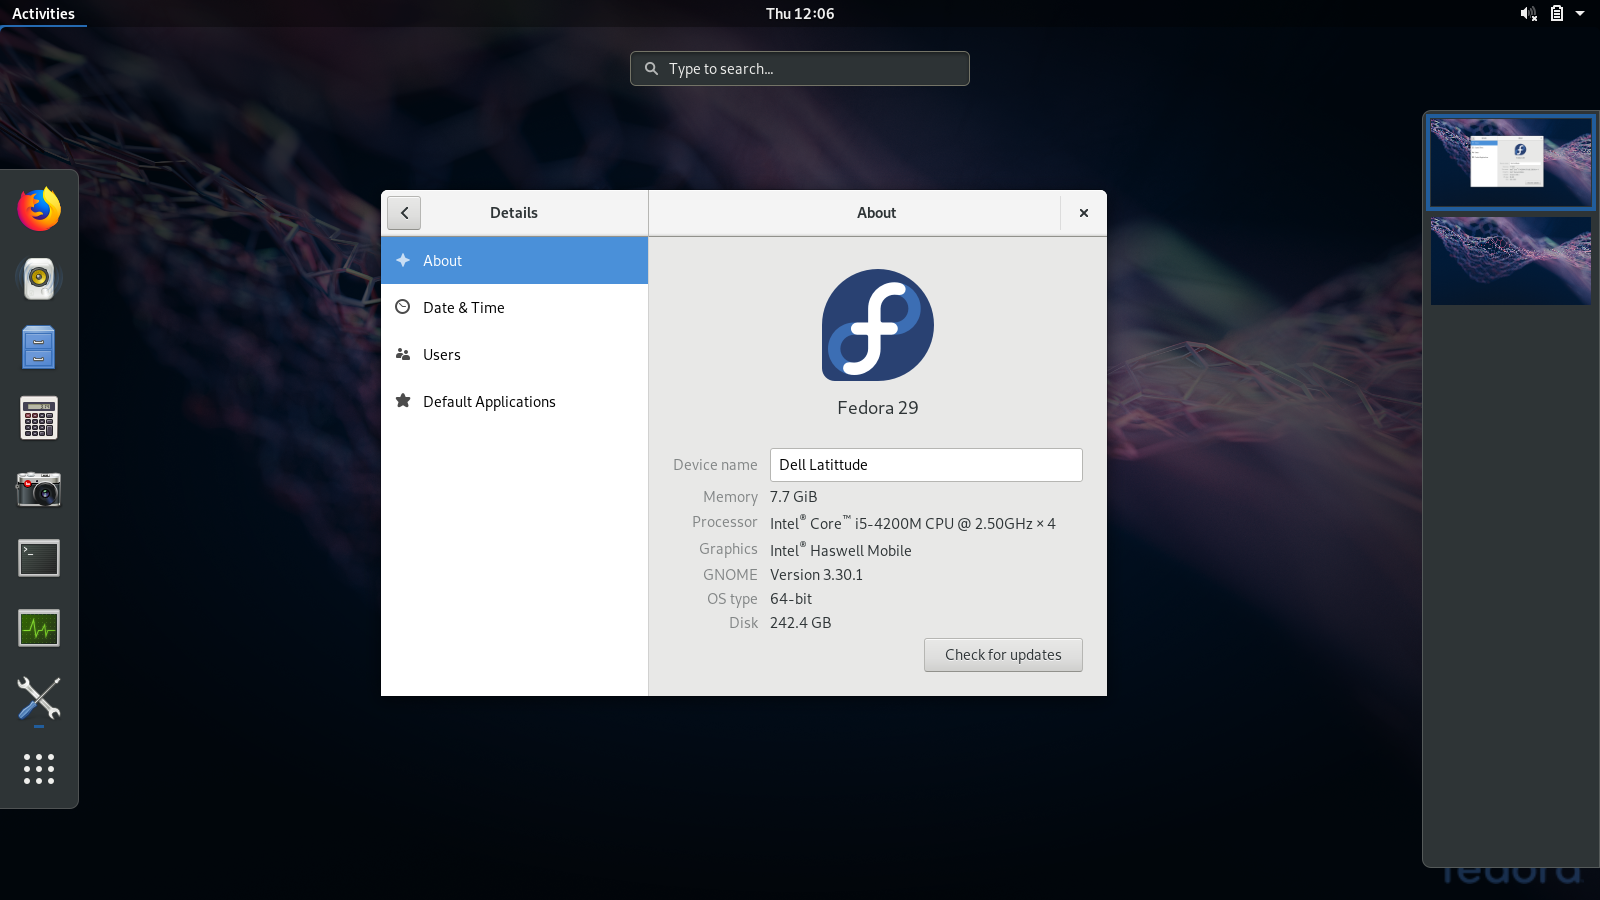
\includegraphics[scale=0.15]{fedora-screenshot.png}
	\end{figure}
	\begin{columns}
		\small
		\begin{column}{0.35\textwidth}
			\begin{itemize}
				\item \textbf{Ease of Use:} Easy
				\item \textbf{Stability:} Somewhat Stable
				\item \textbf{Default DE:} GNOME
			\end{itemize}
		\end{column}
		\begin{column}{0.65\textwidth}
			\small
			\textbf{Description:} Red Hat's desktop distribution that uses more cutting-edge software than Red Hat Enterprise Linux (server distribution).
			\begin{itemize}
				\item Less stable than RHEL and CentOS, but newer software.
				\item Its package manager is \textit{dnf}
			\end{itemize}
		\end{column}
	\end{columns}
\end{frame}

\begin{frame}{
\includegraphics[scale=0.03]{centos-logo.png} CentOS}
	\begin{figure}
		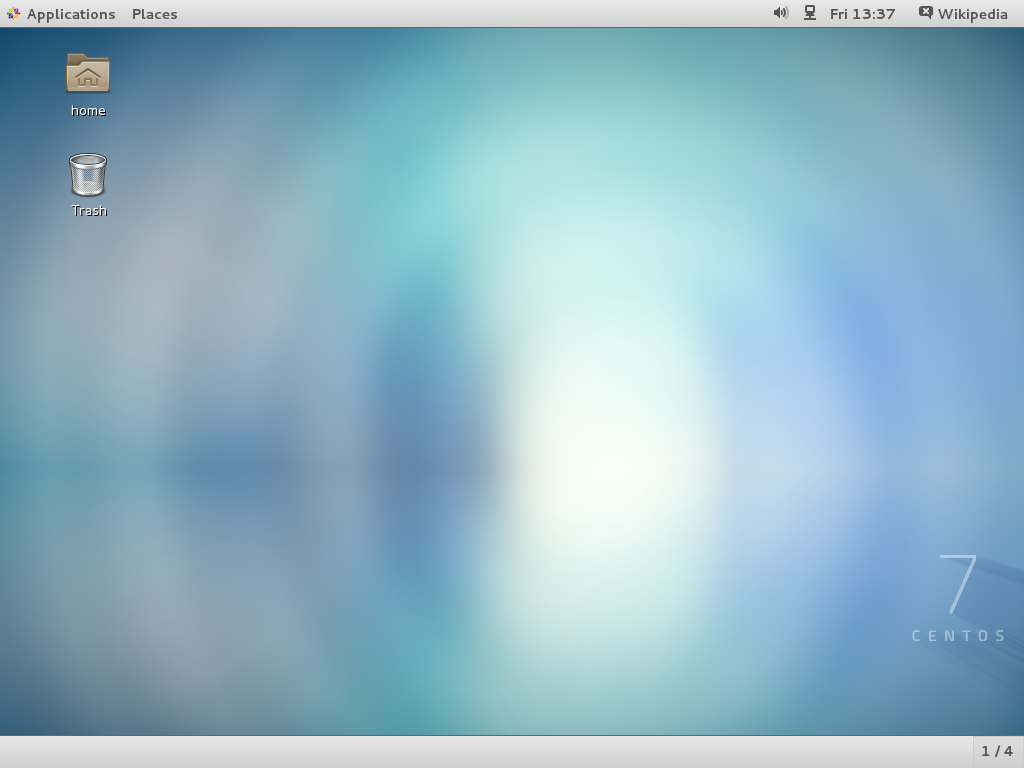
\includegraphics[scale=0.15]{centos-screenshot.png}
	\end{figure}
	\begin{columns}
		\small
		\begin{column}{0.35\textwidth}
			\begin{itemize}
				\item \textbf{Ease of Use:} Medium
				\item \textbf{Stability:} Very Stable
				\item \textbf{Default DE:} GNOME
			\end{itemize}
		\end{column}
		\begin{column}{0.65\textwidth}
			\small
			\textbf{Description:} The Community ENTerprise Operating System of Red Hat, a consumer edition of RHEL.
			\begin{itemize}
				\item Good for server installations, but can still serve as a powerful desktop installation.
				\item Being based off of a server distribution, some things can be complex to set up.
				\item Package manager is \textit{yum}
			\end{itemize}
		\end{column}
	\end{columns}
\end{frame}

\begin{frame}{
\includegraphics[scale=0.07]{opensuse-logo.png} OpenSUSE}
	\begin{figure}
		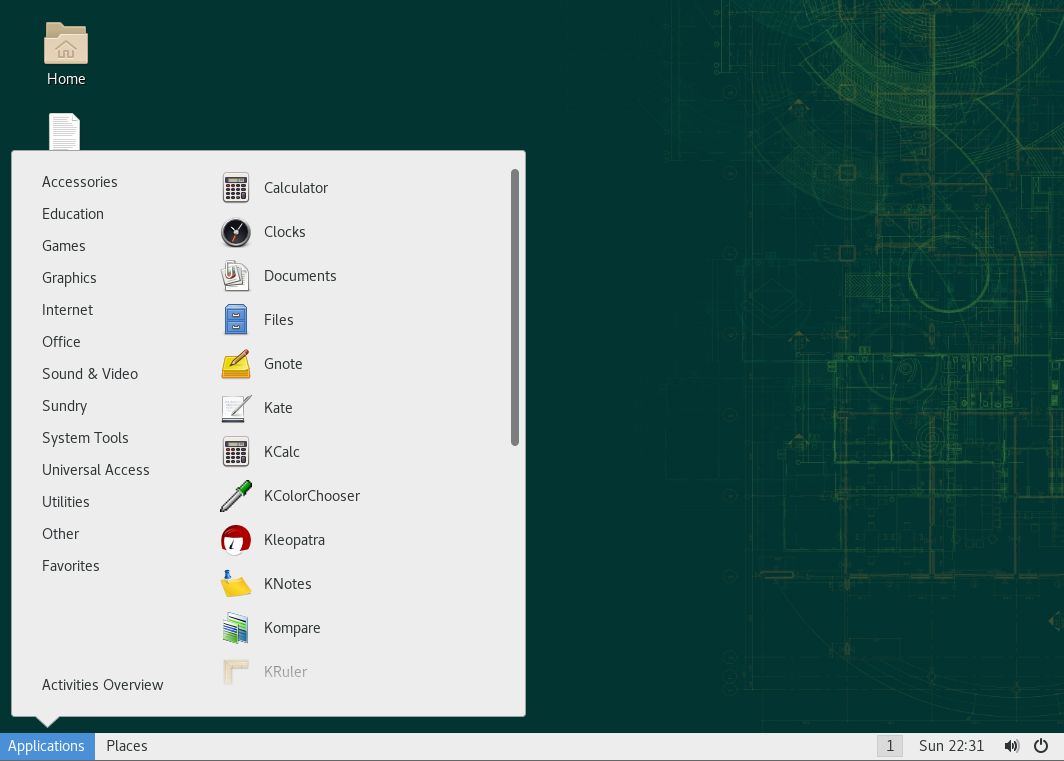
\includegraphics[scale=0.15]{opensuse-screenshot.png}
	\end{figure}
	\begin{columns}
		\small
		\begin{column}{0.35\textwidth}
			\begin{itemize}
				\item \textbf{Ease of Use:} Easy
				\item \textbf{Stability:} Stable (\textit{leap})/Somewhat stable \textit{tumbleweed}
				\item \textbf{Default DE:} GNOME 3 or KDE or manually selectable
			\end{itemize}
		\end{column}
		\begin{column}{0.65\textwidth}
			\small
			\textbf{Description:}  Originally SUSE, sponsored by SUSE Linux GmbH, OpenSUSE a German Linux distro that's used around the world.
			\begin{itemize}
				\item Focus is creating usable open-source tools for software developers and system administrators, while providing a user-friendly desktop and feature-rich server environment.
				\item Package manager is \textit{ZYpp} and \textit{YaST}
			\end{itemize}
		\end{column}
	\end{columns}
\end{frame}

\begin{frame}{
\includegraphics[scale=0.007]{arch-logo.png} Arch Linux}
	\begin{figure}
		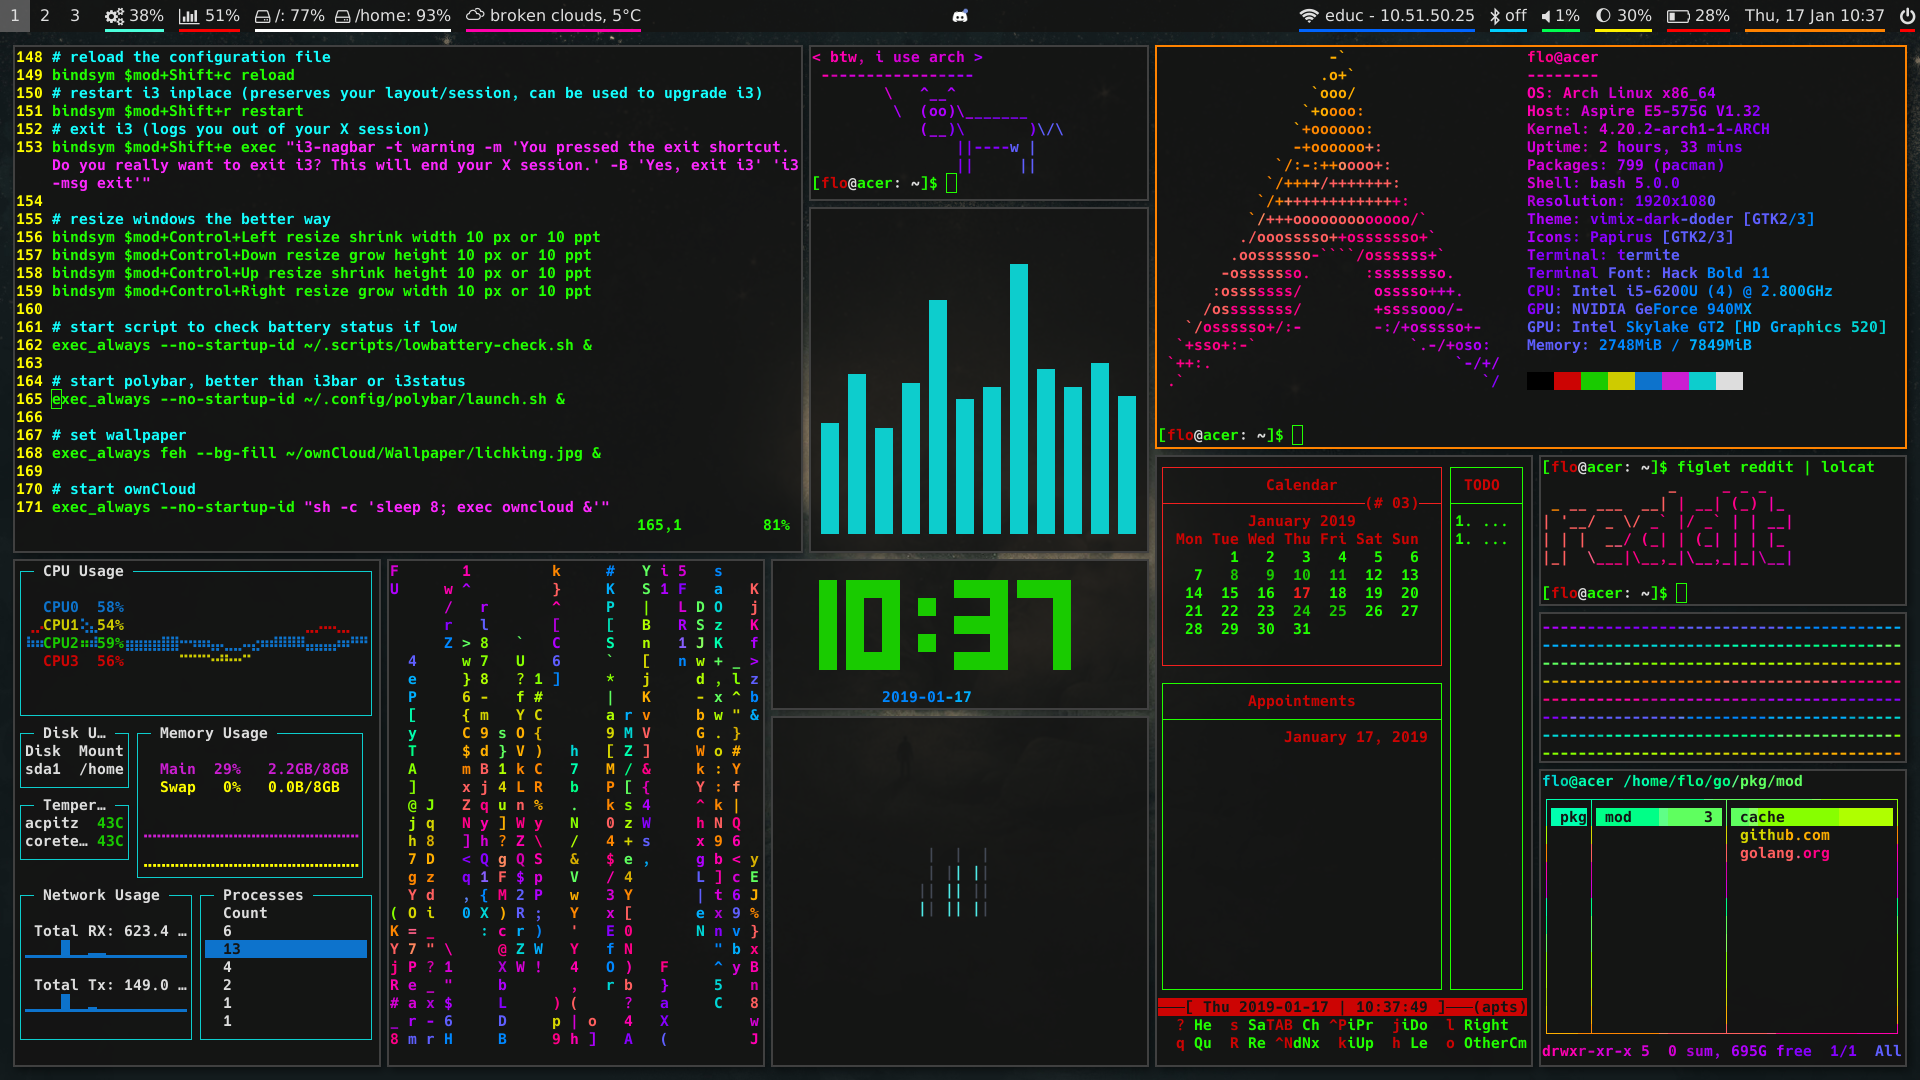
\includegraphics[scale=0.1]{arch-screenshot.png}
	\end{figure}
	\begin{columns}
		\small
		\begin{column}{0.35\textwidth}
			\begin{itemize}
				\item \textbf{Ease of Use:} Difficult
				\item \textbf{Stability:} Varying stability
				\item \textbf{Default DE:} None
			\end{itemize}
		\end{column}
		\begin{column}{0.65\textwidth}
			\small
			\textbf{Description:} Based on the KISS (Keep It Simple, Stupid) principle; a lightweight, flexible, and very customizable Linux distribution.
			\begin{itemize}
				\item User-\textit{centric} rather than user-\textit{friendly}
				\item The system can be as minimal or as maximal as the user desires.
				\item Targeted at experienced Linux users
				\item Package manager is \textit{pacman}
			\end{itemize}
		\end{column}
	\end{columns}
\end{frame}

\begin{frame}{
\includegraphics[scale=0.07]{gentoo-logo.png} Gentoo}
	\begin{figure}
		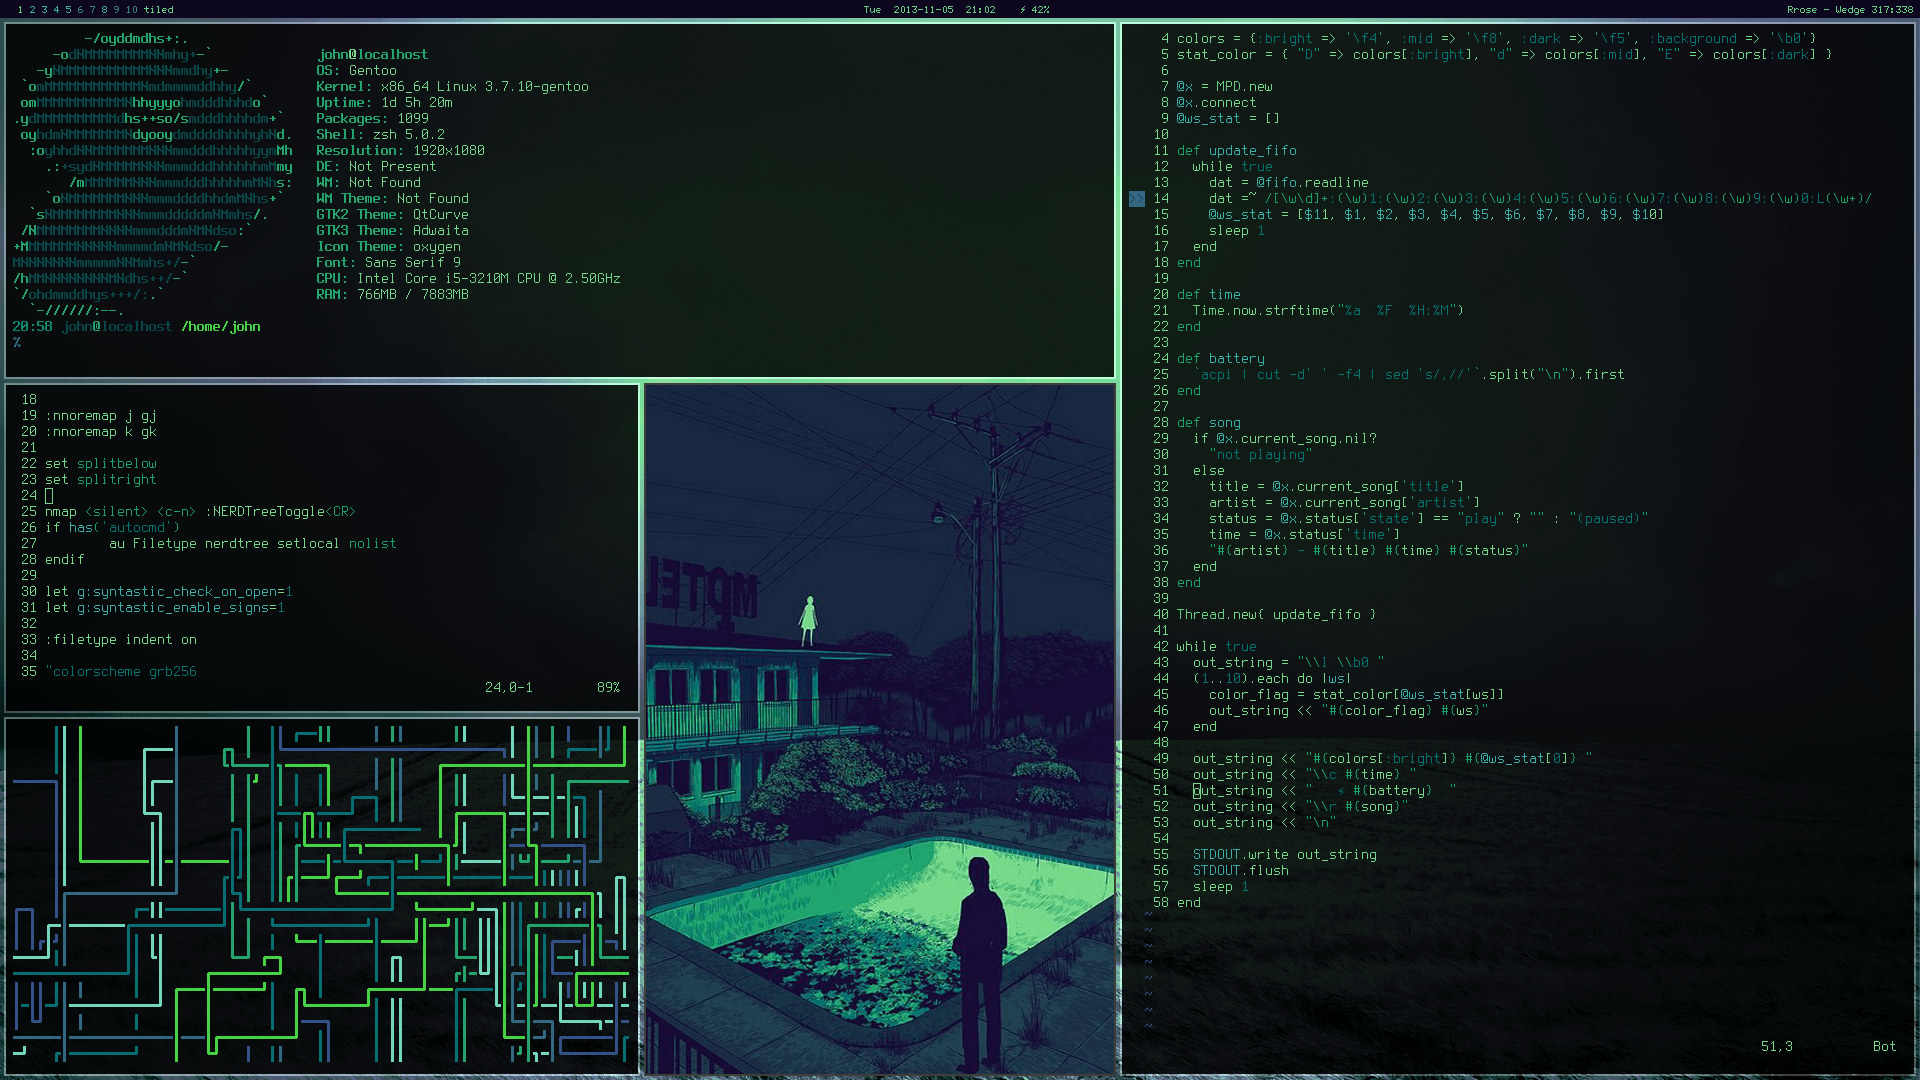
\includegraphics[scale=0.1]{gentoo-screenshot.png}
	\end{figure}
	\begin{columns}
		\small
		\begin{column}{0.35\textwidth}
			\begin{itemize}
				\item \textbf{Ease of Use:} Difficult
				\item \textbf{Stability:} Varying Stability
				\item \textbf{Default DE:} None
			\end{itemize}
		\end{column}
		\begin{column}{0.65\textwidth}
			\small
			\textbf{Description:} Named after the fastest species of penguin, Gentoo requires all software to be compiled locally for performance, optimized for your specific machine.
			\begin{itemize}
				\item A DIY distro like Arch
				\item The next level of full control over your operating system.
				\item Package manager is \textit{portage}
			\end{itemize}
		\end{column}
	\end{columns}
\end{frame}

\begin{frame}{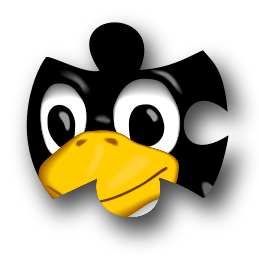
\includegraphics[scale=0.07]{lfs-logo.png} Linux From Scratch (LFS)}
	\begin{figure}
		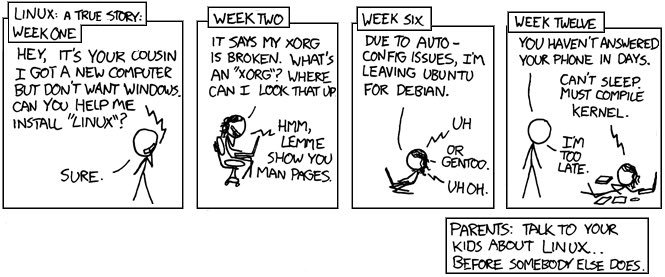
\includegraphics[scale=0.3]{xkcd.jpg}
	\end{figure}
	\begin{columns}
		\small
		\begin{column}{0.35\textwidth}
			\begin{itemize}
				\item \textbf{Ease of Use:} Very Difficult
				\item \textbf{Stability:} Depends on your skillage!
				\item \textbf{Default DE:} Whatever you feel like, baby!
			\end{itemize}
		\end{column}
		\begin{column}{0.65\textwidth}
			\small
			\textbf{Description:} A project that provides you with step-by-step instructions for building your own custom Linux system, entirely from source code.
			\begin{itemize}
				\item Want to make your own Linux distribution? This is how!
				\item {\color{blue}\url{ http://www.linuxfromscratch.org/}}
				\item {\color{blue}\url{https://github.com/ASULUG/Linux-Fom-Scratch}}
			\end{itemize}
		\end{column}
	\end{columns}
\end{frame}

\begin{frame}{Addendum}
	\begin{itemize}
		\item There are embedded Linux distributions as well:
		\begin{itemize}
			\item \textbf{Raspbian:} for the ARM architecture on Raspberry Pi
			\item \textbf{octo:} for IoT devices
		\end{itemize}
		\item For Chromebook: GalliumOS
		\item \url{https://reddit.com/r/unixporn} - Do it. You'll be inspired.
	\end{itemize}
	~\\
	\textbf{\LARGE ASULUG Resources:}
	\begin{itemize}
		\item \textbf{GitHub:} \url{https://github.com/ASULUG/}
		\item \textbf{YouTube:} \url{https://www.youtube.com/channel/UCaXljzLXzFFpZfGOr-Uu6cw}
		\item \textbf{Twitch:} \url{https://www.twitch.tv/asulug}
	\end{itemize}
\end{frame}

\begin{frame}{Feedback!}
	\begin{figure}
		
\includegraphics[scale=0.5]{qr-code.png}
		\caption{\url{https://goo.gl/forms/gbHOa0j5SBjZdMW13}}
	\end{figure}
\end{frame}
\end{document}